\documentclass[twoside,10pt,a4paper]{article}

%================================ PREAMBLE ==================================

%--------- Packages -----------
\usepackage{fullpage}
\usepackage{amssymb}
\usepackage{amsmath}
\usepackage{amsthm}
\usepackage{latexsym}
\usepackage{graphicx}
\usepackage{color}
\usepackage{hyperref}
%\usepackage{algorithm,algorithmic}

%----------Spacing-------------
\setlength{\oddsidemargin}{0.25 in}
\setlength{\evensidemargin}{-0.25 in}
\setlength{\topmargin}{-0.6 in}
\setlength{\textwidth}{6.5 in}
\setlength{\textheight}{9.4 in}
\setlength{\headsep}{0.75 in}
\setlength{\parindent}{0 in}
\setlength{\parskip}{0.1 in}

%----------Header--------------
\newcommand{\assignmentreport}[4]{
   \pagestyle{myheadings}
   \thispagestyle{plain}
   \newpage
   \setcounter{page}{1}
   \noindent
   \begin{center}
   \framebox{
      \vbox{\vspace{2mm}
    \hbox to 6.28in { {\bf E0 270 Machine Learning} \hfill {\it Due:} #2 }
       \vspace{6mm}
       \hbox to 6.28in { \hfill {\Large Assignment #1 - Report} \hfill }
       \vspace{6mm}
       \hbox to 6.28in {{\it #3} \hfill {\it #4} }
      \vspace{2mm}}
   }
   \end{center}
   \markboth{Assignment #2 :\it #3,\it#4}{Assignment #2: \it #3,\it#4}
   \vspace*{4mm}
}

%--------Environments----------
\theoremstyle{definition}
\newtheorem{thm}{Theorem}[section]
\newtheorem{lem}[thm]{Lemma}
\newtheorem{prop}[thm]{Proposition}
\newtheorem{cor}[thm]{Corollary}
\newenvironment{pf}{{\noindent\sc Proof. }}{\qed}
\newenvironment{map}{\[\begin{array}{cccc}} {\end{array}\]}

\theoremstyle{definition}
\newtheorem*{defn}{Definition}
\newtheorem{exmp}{Example}
\newtheorem*{prob}{Problem}
\newtheorem*{exer}{Exercise}

\theoremstyle{remark}
\newtheorem*{rem}{Remark}
\newtheorem*{note}{Note}

%---------Definitions----------
\newcommand{\Fig}[1]{Figure~\ref{#1}}
\newcommand{\Sec}[1]{Section~\ref{#1}}
\newcommand{\Tab}[1]{Table~\ref{#1}}
\newcommand{\Tabs}[2]{Tables~\ref{#1}--\ref{#2}}
\newcommand{\Eqn}[1]{Eq.~(\ref{#1})}
\newcommand{\Eqs}[2]{Eqs.~(\ref{#1}-\ref{#2})}
\newcommand{\Lem}[1]{Lemma~\ref{#1}}
\newcommand{\Thm}[1]{Theorem~\ref{#1}}
\newcommand{\Cor}[1]{Corollary~\ref{#1}}
\newcommand{\App}[1]{Appendix~\ref{#1}}
\newcommand{\Def}[1]{Definition~\ref{#1}}
%
\renewcommand{\>}{{\rightarrow}}
\newcommand{\R}{{\mathbb R}}
\newcommand{\Z}{{\mathbb Z}}
\newcommand{\N}{{\mathbb N}}
\renewcommand{\P}{{\mathbf P}}
\newcommand{\E}{{\mathbf E}}
\newcommand{\Var}{{\mathbf{Var}}}
\newcommand{\I}{{\mathbf I}}
\newcommand{\1}{{\mathbf 1}}
\newcommand{\0}{{\mathbf 0}}
\renewcommand{\H}{{\mathcal H}}
\newcommand{\F}{{\mathcal F}}
\newcommand{\G}{{\mathcal G}}
\renewcommand{\L}{{\mathcal L}}
\newcommand{\cN}{{\mathcal N}}
\newcommand{\X}{{\mathcal X}}
\newcommand{\Y}{{\mathcal Y}}
\newcommand{\sign}{\textup{\textrm{sign}}}
\newcommand{\er}{\textup{\textrm{er}}}
\newcommand{\abs}{\textup{\textrm{abs}}}
\newcommand{\sq}{\textup{\textrm{sq}}}
\newcommand{\zo}{\textup{\textrm{0-1}}}
\newcommand{\hinge}{\textup{\textrm{hinge}}}
\newcommand{\ramp}{\textup{\textrm{ramp}}}
\newcommand{\mar}{\textup{\textrm{margin}}}
\newcommand{\lin}{\textup{\textrm{lin}}}
\newcommand{\poly}{\textup{\textrm{poly}}}
\newcommand{\majority}{\textup{\textrm{majority}}}
\newcommand{\maj}{\textup{\textrm{maj}}}
\newcommand{\co}{\textup{\textrm{co}}}
\newcommand{\agg}{\textup{\textrm{agg}}}
\newcommand{\bad}{\textup{\textrm{bad}}}
\newcommand{\EX}{\textup{\textrm{\textit{EX}}}}
\newcommand{\GD}{\textup{\textrm{{GD}}}}
\newcommand{\EG}{\textup{\textrm{{EG}}}}
\newcommand{\algorithm}{\textup{\textrm{{algorithm}}}}
\newcommand{\VCdim}{\textup{\textrm{{VCdim}}}}
\newcommand{\VCentropy}{\textup{\textrm{{VC-entropy}}}}
\newcommand{\Pdim}{\textup{\textrm{{Pdim}}}}
\newcommand{\fat}{\textup{\textrm{{fat}}}}
\newcommand{\x}{{\mathbf x}}
\newcommand{\w}{{\mathbf w}}
\newcommand{\p}{{\mathbf p}}
\newcommand{\q}{{\mathbf q}}
\renewcommand{\r}{{\mathbf r}}
\renewcommand{\u}{{\mathbf u}}
\renewcommand{\b}{{\mathbf b}}
\newcommand{\bloss}{{\boldsymbol \ell}}
\newcommand{\balpha}{{\boldsymbol \alpha}}
\newcommand{\bxi}{{\boldsymbol \xi}}
\newcommand{\bpsi}{{\boldsymbol \psi}}
\newcommand{\btau}{{\boldsymbol \tau}}

%=============================== END PREAMBLE ===============================

%============================ BEGIN DOCUMENT ================================
\begin{document}

%Use the following format: \assignmentreport{Assignment number}{Due date}{Your name}{SR Number}

\assignmentreport{3}{Feb 28, 2012}{Sachin Nagargoje}{04-04-00-10-41-11-1-08449}

%-----------------------

\section{Solution: Problem 1}
Part (1) \\
Refer to Code \\

Part (2)\\
\begin{center}
figure for 1a \hspace{180pt} figure for 1b \\
\scalebox{0.35}{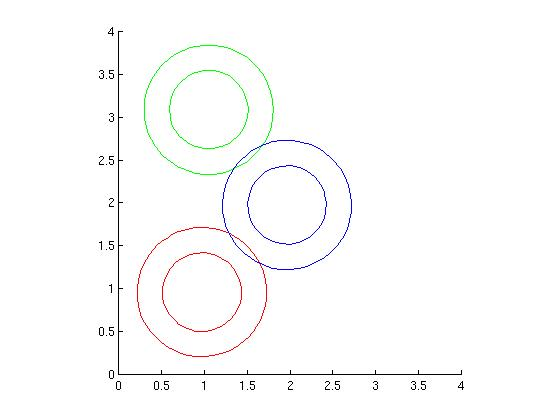
\includegraphics{./Problem1/1a2} }
\scalebox{0.35}{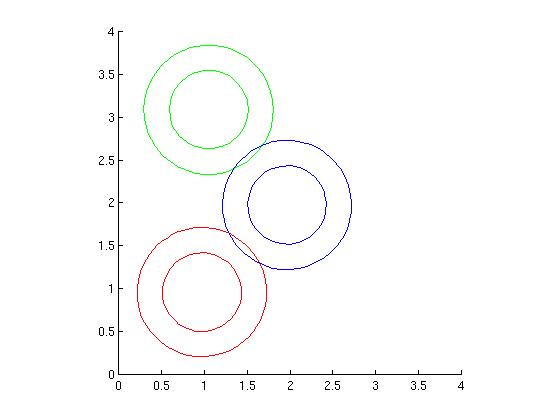
\includegraphics{./Problem1/1b2} } \\

figure for 1c \hspace{180pt} figure for 2a \\
\scalebox{0.35}{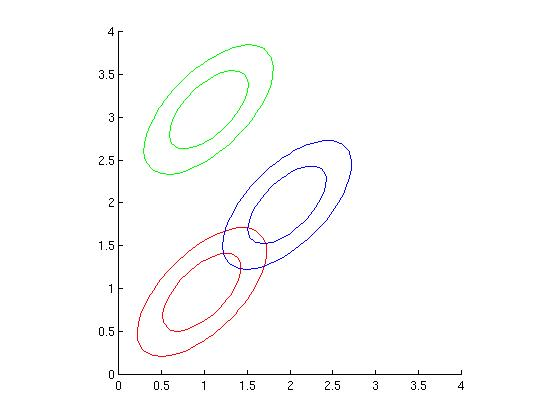
\includegraphics{./Problem1/1c2} }
\scalebox{0.35}{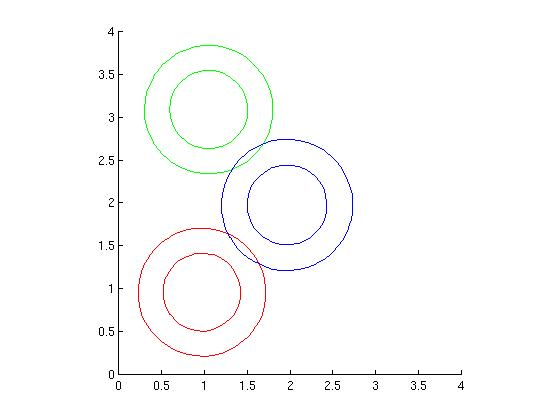
\includegraphics{./Problem1/2a2} } \\
\end{center}

\newpage

\begin{center}
figure for 2b \hspace{180pt} figure for 2c \\
\scalebox{0.35}{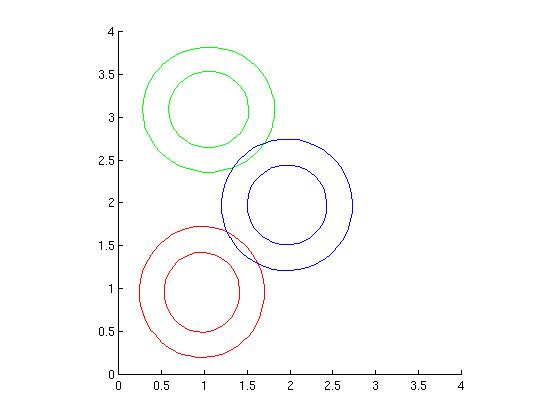
\includegraphics{./Problem1/2b2} }
\scalebox{0.35}{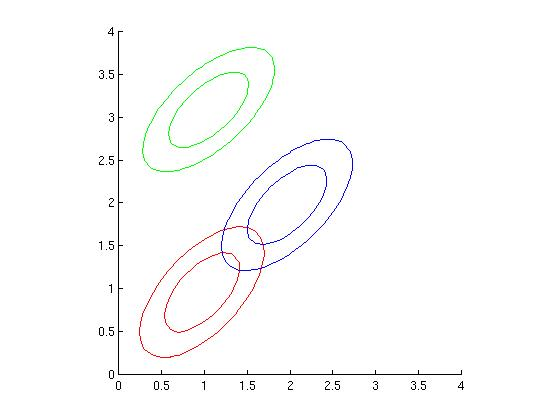
\includegraphics{./Problem1/2c2} } \\
\end{center}

Part (3) \\
\begin{center} 
figure for 1c \hspace{180pt} figure for 2c \\
\scalebox{0.35}{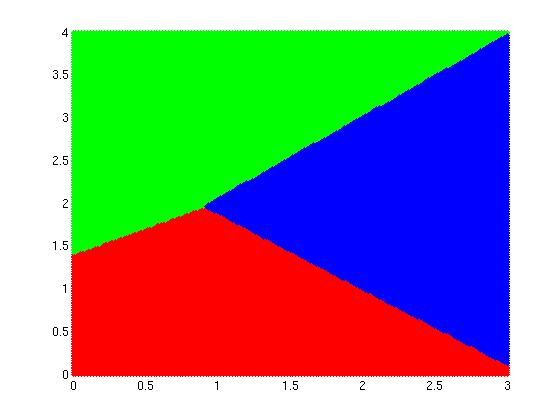
\includegraphics{./Problem1/1c1} }
\scalebox{0.35}{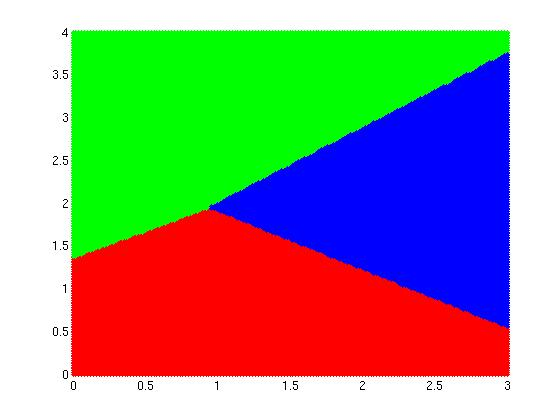
\includegraphics{./Problem1/2c1} } \\
\end{center}
In case of 1c, that is shared covariance matrix, the decision boundary is linear due to the shared covariance matrix.\\
Due to the shared covariance matrix, the quadratic term in the classifier cancels out and we get a linear decision boundary.\\
In case of 2c , where each class have different covariance matrix, this term remains in the classifier making the decision boundary non-linear.\\

\newpage
Part (4) \\
\begin{center} 
\scalebox{0.4}{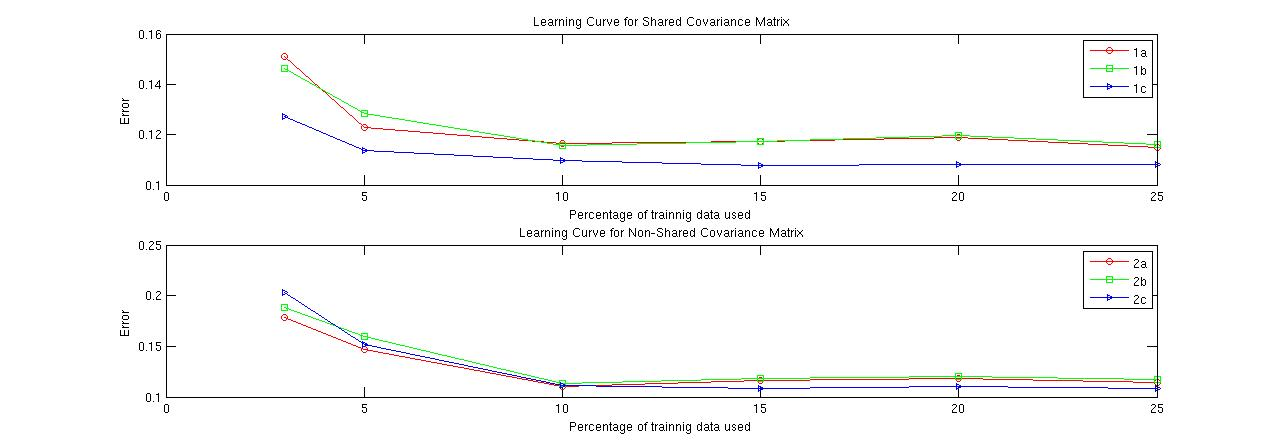
\includegraphics{./Problem1/4} } \\
In both the cases , the error reduces as we increase the number of training data.
\end{center}

\end{document}

%=========================== END DOCUMENT ==============================

